\section{Aluminiumoxid-ALD}
\label{aluminaald}

Einen Vorzeige-Prozess für Atomlagenabscheidungen bildet die Abscheidung von Aluminiumoxid \ce{Al2O3}, für die häufig das Precursorpaar Trimethylaluminium (TMA, \ce{Al(CH3)3}) und Wasser genutzt wird\cite{puurunen_surface_2005}.
Aufgrund seiner relativ hohen Dielektrizitätskonstanten von $k\approx 8$ ersetzt \ce{Al2O3} langsam gemeinsam mit Materialien wie \ce{HfO2} und \ce{ZrO2}\cite{smith_chemical_2000} das gebräuchliche Siliziumdioxid ($k=3.9$) als Dielektrikum in der Halbleiterindustrie, wird aber auch häufig zur Herstellung passivierender Schichten eingesetzt\cite{yun_passivation_2004,poodt_high-speed_2010}.
Deshalb soll der TMA-\ce{H2O}-Prozess im Folgenden besonders hinsichtlich der Reaktion der Precursormoleküle mit der Oberfläche untersucht werden.

Dazu wurden verschiedene Parametersätze hinsichtlich der Anwendbarkeit auf reaktive Oberflächenabscheidungen untersucht, und schließlich erste Oberflächenreaktionen mit ihnen simuliert.
Dabei ist bisher lediglich die Simulation der reaktiven Hydroxylierung der Oberfläche gelungen, was auf die mangelhafte Beschreibung der \ce{Al-C}-Bindungen mit den benutzten Potentialen zurück zu führen ist.

\subsection{ReaxFF-Parametersätze}

Für die MD-Simulation von \ce{Al2O3} stehen drei Parametrisierungen zur Verfügung, die bereits aus den Untersuchungen der Silizium-Potentiale bekannt sind (Abschnitt~\ref{siliconpvd}):

\pot{Al\_Al0\_AlN} aus LAMMPS\cite{plimpton_lammps_2014}, \pot{liu\_ettringite}\cite{liu_development_2012}, welches nachfolgend nur als \pot{liu} geführt werden soll, und \pot{narayanan}\cite{narayanan_reactive_2012}.
Ihnen ist gemein, dass sie ausgehend von Silizium-Parametrisierungen um Parameter für Aluminium-Verbindungen erweitert wurden, weshalb sie auch im vorherigen Kapitel untersucht wurden.
Auf eine Bewahrung der Konsistenz der Siliziumparameter wurde dabei scheinbar verzichtet, sodass etwa mit der \pot{liu}-Parametrisierung eine verlässliche Simulation von Silizium-Verbindungen verhindert, im Gegenzug aber die Simulation von Aluminium-Verbindungen ermöglicht wird.
Eine Kombination verschiedener Parametrisierungen ist zwar denkbar und wird bereits kommerzieller Software durchgeführt\cite{biovia_materials_2014}, würde aber für die vorliegenden Potentiale höchstens zweifelhafte Verbesserungen bringen.

Die \pot{Al\_Al0\_AlN}-Datei stammt direkt aus der offiziellen LAMMPS-Distribution\cite{plimpton_lammps_2014}, wurde jedoch am 17. Mai 2013 während der Ergänzung von Referenzen auf wissenschaftliche Publikationen in anderen Parameterdateien kommentarlos aus dem Paket entfernt\cite{thompson_lammps_2013}.
Bei den Recherchen konnte kein Hinweis auf das ursprüngliche Anwendungsgebiet gefunden werden, weshalb mit diesen Parametern berechnete Eigenschaften mit Vorsicht überprüft werden.

Das \pot{liu}-Potentialdatei wurde für die Simulation von Ettringit (\ce{Ca6[Al(OH)6]2(SO4)3 26H2O}) erstellt, welches \ce{Al-O}-Bindungen und \ce{OH}-Gruppen enthält, sodass zumindest die Simulation des Bulkmaterials und einer hydroxylierten Oberfläche aussichtsreich erscheint.
Sie beschreibt die Oberflächenhydroxylierung und stellt sich daher als Favorit für Parsivald-Simulationen heraus, obwohl ihr eigentliches Anwendungsgebiet auf der Simulation von Kristallen liegt.

Zuletzt steht die \pot{narayanan}-Parametrisierung für \ce{Li-Al}-Silikate, insbesondere zur Simulation von Eukryptit (\ce{LiAl[SiO4]}), zur Verfügung, lässt aber keine endgültige Aussage über die Qualität der \ce{Al-O}-Bindungen und \ce{OH}-Gruppen zu.
Zwar besteht ihr Trainingssatz aus verschiedenen Lithium-Aluminium-Kristallen, aber nur $\gamma$-\ce{LiAlO2} beinhaltet direkte \ce{Al-O}-Bindungen, wo hingegen keine der Strukturen Hydroxylgruppen beinhaltet.
Es ist daher unwahrscheinlich, dass die \pot{narayanan}-Potentialdatei komplizierte Systeme verlässlich darstellt.

\subsection{Voruntersuchungen}

Wie in den vorherigen Abschnitten werden hier separate Voruntersuchungen durchgeführt, zu denen die Reaktion von Precursormolekülen mit der Oberfläche ergänzt wurde.
Die Referenzwerte sind in Anhang~\ref{appendix_constants} zusammen gefasst.

\subsubsection{Vergleich der strukturellen Eigenschaften von \texorpdfstring{\ce{Al2O3}}{Al2O3}}

Zum Vergleich der strukturellen Eigenschaften des Bulkmaterials wurde in MD-Simulationen ein $\alpha$-\ce{Al2O3}-Kristall bei \SI{1500}{\kelvin} für \num{100000} Zeitschritte isotherm-isobar relaxiert und vor den abschließenden Messungen auf Raumtemperatur herunter gekühlt.
Die Abkühlung wurden versehentlich um einen Faktor 10 zu schnell durchgeführt, weshalb die beobachteten Dichten vermutlich leicht unterschätzt sind.
Eine erneute Berechnung der Werte steht noch aus, doch zeigen sich anhand der Dichten der amorpher Strukturen genügend Hinweise auf die Anwendbarkeit der Parametrisierungen.
Referenzwerte der Dichten für unterschiedliche Temperaturen liegen bei \SI{3.99}{\gpcc} bei Raumtemperatur und \SI{3.80}{\gpcc} bei \SI{1500}{\kelvin}\cite{fiquet_high-temperature_1999}.
Bindungslängen und Koordinationszahlen wurden direkt aus der RDF der kristallinen Strukturen nach der Relaxation bestimmt.
Ihre Referenzwerte wurden auf die gleiche Weise durch die Untersuchung der idealen Kristallstruktur bestimmt, welche mittels Materials Studio\cite{biovia_materials_2014} auf Basis eines $\alpha$-\ce{Al2O3}-Kristalles präpariert wurde, wobei die Kristallstruktur und Gitterkonstante nach experimentellen Werten gewählt wurden\cite{haynes_crc_2011}.

\begin{table}[b!]
  \oddrowcolors
  \caption[Vergleich struktureller Eigenschaften von $\alpha$-\ce{Al2O3}]{
    Vergleich struktureller Eigenschaften von \ce{Al2O3} für verfügbare ReaxFF-Parametrisierungen.
    Referenzwerte stammen von einer relaxierten Kristallstruktur.
  }
  \label{tab:aluminabulks}

  \begin{tabularx}{\textwidth}{|Xllll|}
    \hline
    \textbf{Eigenschaft}                & \textbf{Referenz}    & \textbf{\pot{Al\_Al0\_AlN}} & \textbf{\pot{liu}}   & \textbf{\pot{narayanan}} \\
    \hline
    Dichte, $\alpha$-kristallin         & \SI{3.98}{\gpcc}     & \SI{4.31}{\gpcc}            & \SI{3.88}{\gpcc}     & \SI{3.76}{\gpcc}         \\
    Dichte, amorph                      & \SI{>3.2}{\gpcc}     & ~                           & \SI{3.66}{\gpcc}     & \SI{2.93}{\gpcc}         \\
    \ce{Al-O}-Bindungslänge, kristallin & \SI{1.90}{\angstrom} & \SI{1.94}{\angstrom}        & \SI{1.88}{\angstrom} & \SI{1.85}{\angstrom}     \\
    \ce{Al-O}-Koordination, kristallin  & \num{4.00}           & \num{5.40}                  & \num{4.55}           & \num{4.05}               \\
    \ce{Al-Al}-Koordination, kristallin & \num{4.00}           & \num{6.66}                  & \num{5.98}           & \num{5.10}               \\
    \ce{O-O}-Koordination, kristallin   & \num{12.0}           & \num{12.4}                  & \num{11.0}           & \num{12.2}               \\
    \hline
  \end{tabularx}
\end{table}

Für die Bestimmung der Dichte der amorphen Struktur wurde das Bulkmaterial über den Schmelzpunkt von \SI{2317}{\kelvin} auf \SI{2555}{\kelvin} erhitzt, bei dieser Temperatur relaxiert und langsam auf Raumtemperatur abgekühlt.
Aufgrund der strukturellen Vielfalt bei amorphen Aluminiumoxiden liegt der Referenzbereich der Dichte von gasphasen-abgeschiedenen \ce{Al2O3}-Schichten zwischen \SI{3.2}{\gpcc} und \SI{3.9}{\gpcc}\cite{wang_dependence_1997}.

Die Verteilung der Koordinationszahlen amorpher Schichten wurde in dieser Arbeit nicht näher untersucht, da einerseits nur Vergleiche mit anderen MD-Rechnungen zur Verfügung stehen\cite{gutierrez_molecular_2002}, andererseits ein weiteres eigenes Werkzeug hätte geschrieben und getestet werden müssen.
Die Integration eines solchen Werkzeuges zur Bestimmung der Verteilung der Koordinationen in Parsivald könnte allerdings helfen, die Struktur der Schicht während der laufenden Simulation zu untersuchen.

Die Ergebnisse dieser Untersuchungen (Tabelle~\ref{tab:aluminabulks}) zeichnen ein vielseitiges Bild.
Einerseits stimmt die kristalline Bindungslänge für alle Parametrisierungen bis auf \SI{3}{\percent} überein, andererseits ergeben sich große Unterschiede in der Dichte der Kristalle, die durch die Verformung der Kristallstrukturen verursacht wird.
Im Fall von \pot{Al\_Al0\_AlN} weicht die kristalline Dichte um \SI{+8.3}{\percent} ab und übersteigt die Dichte der dichtesten \ce{Al2O3}-Kristalle bei Normaldruck, wie sich auch an den erhöhten Koordinationszahlen zeigt.
Die beiden verbleibenden Parametersätze \pot{liu} und \pot{narayanan} zeigen geringere Dichten von \SI{3.88}{\gpcc} und \SI{3.76}{\gpcc}, doch zeigen Abweichungen der Koordinationszahlen erste Verformungen der Kristallstrukturen an.
%% die noch oberhalb der Dichte von $\gamma$-\ce{Al2O3} (\SI{3.67}{\gpcc}\cite{dynys_alpha_1982}) liegt.

Eine Bestimmung der amorphen Dichten für die \pot{liu}- und \pot{narayanan}-Parametersätze zeigt für \pot{liu} mit \SI{3.66}{\gpcc} eine amorphe Dichte im erwarteten Bereich, während \pot{narayanan} bei allen Simulationen eine Dichte von \SI{2.93}{\gpcc} erreicht und damit unterhalb der beobachteten Werte liegt, obwohl es die beste Koordination für kristalline Strukturen zeigt.

Damit ist die \pot{liu}-Parametrisierung erfolgreich bei der Darstellung von Kristallen und amorphen Bulkstrukturen von \ce{Al2O3}.

\subsubsection{Simulationen der Stabilität von Precursormolekülen}

Die Stabilität für Trimethylaluminium (TMA) wurde nach dessen manueller Präparation für die drei Parametersätze \pot{Al\_Al0\_AlN}, \pot{liu\_ettringite} (kurz \pot{liu}) und \pot{narayanan} untersucht (Abbildung~\ref{fig:tmastability}).
Die Strukturdaten von TMA\cite{haynes_crc_2011} sind in Anhang~\ref{appendix_constants} zusammen gefasst.

Mit den \pot{Al\_Al0\_AlN}-Parametern konnte TMA stabil simuliert werden (Abbildung~\ref{fig:tmamonomer}), jedoch nehmen die simulierten Moleküle nicht die erwartete planare Struktur ein, sondern weisen eine trigonal-pyramidale Struktur mit leicht reduzierten \ce{C-Al-C}-Bindungs\-winkeln von durchschnittlich \SI{103}{\degree} auf.
Die Bindungslängen stimmen hingegen mit durchschnittlich \SI{2.020}{\angstrom} (Referenz: \SI{1.957}{\angstrom}\cite{haynes_crc_2011}) für \ce{Al-C} und \SI{1.106}{\angstrom} (Referenz: \SI{1.113}{\angstrom}\cite{haynes_crc_2011}) für \ce{C-H} bis auf \SI{3}{\percent} mit Referenzwerten überein.
Mit dieser Parametrisierung konnte ebenfalls das TMA-Dimer bei niedrigen Temperaturen simuliert werden (Abbildung~\ref{fig:tmadimer}).

\begin{figure}[b!]
  \captionsetup[subfigure]{singlelinecheck=false}

  \vspace{1em}

  \begin{subfigure}[t]{4cm}
    \begin{overpic}[width=\textwidth]{tma_Al}
      \put(20,100){
        \begin{minipage}{4.7cm}
          \begin{framed}
            \chemlegendce{Al}
            \hspace{0.5em}
            \chemlegendce{C}
            \hspace{0.5em}
            \chemlegendce{H}
          \end{framed}
        \end{minipage}
      }
    \end{overpic}
    \subcaption{
      \pot{Al\_Al0\_AlN}: \\
      stabiles TMA
    }
    \label{fig:tmamonomer}
  \end{subfigure}
  \hfill
  \begin{subfigure}[t]{5.5cm}
    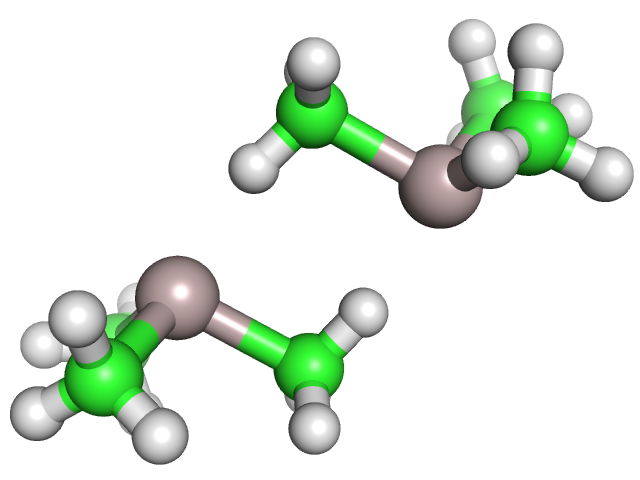
\includegraphics[width=\textwidth]{tma_Al_dimer}
    \subcaption{
      \pot{Al\_Al0\_AlN}: \\
      stabiles TMA-Dimer
    }
    \label{fig:tmadimer}
  \end{subfigure}
  \hfill
  \begin{subfigure}[t]{4.5cm}
    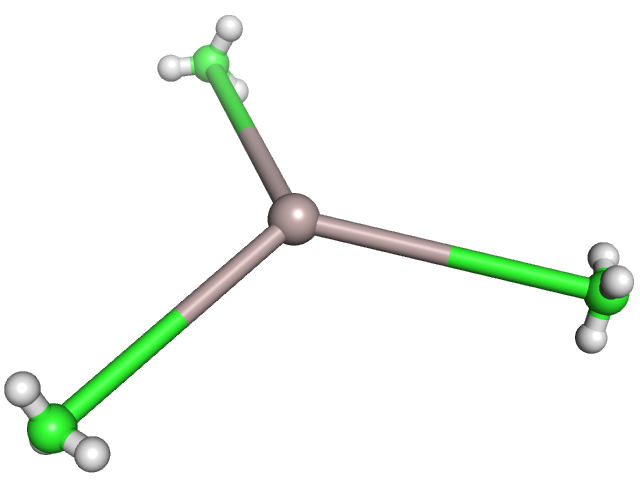
\includegraphics[width=\textwidth]{tma_liu}
    \subcaption{
      \pot{liu\_ettringite}: \\
      Keine \ce{Al-C}-Bindungen
    }
    \label{fig:tmaliu}
  \end{subfigure}

  \caption{Stabilität der TMA-Moleküle für verschiedene ReaxFF-Parametersätze}
  \label{fig:tmastability}
\end{figure}

TMA-Simulationen mit dem \pot{liu}-Parametersatz zeigen hingegen keinen Erfolg, da er keine \ce{Al-C}-Bindungen beschreibt.
Somit lösen sich in den Simulationen ungebundene Methylgruppen vom zentralen Aluminium-Atom (Abbildung~\ref{fig:tmaliu}).
Die \pot{narayanan}-Parametrisierung verfügt über keine Kohlenstoff-Parameter und kann deshalb nicht für TMA-Simulationen genutzt werden.

Simulationen von Wassermolekülen waren hingegen mit allen Parametrisierungen erfolgreich.
Anhand des \pot{Al\_Al0\_AlN}-Parametersatzes wurden auch Simulationen der Reaktionen zwischen TMA und Wasser in der Gasphase versucht, wie sie beispielsweise bei Vermischung der Precursorgase im ALD-Reaktor auftreten können.
Diese zeigten keinen Erfolg, da die \ce{Al-C}-Bindungen in der \pot{Al\_Al0\_AlN}-Parametrisierung entweder zu stark sind oder in zu großem Maß von den Methylgruppen abgeschirmt werden.

TMA lässt sich also mit dem \pot{liu}-Parametersatz und der \pot{narayanan}-Parametrisierung nicht simulieren.
Der \pot{Al\_Al0\_AlN}-Parametersatz kann hingegen weder das Bulkmaterial noch die spontane Reaktionen zwischen beiden Precursorgasen beschreiben.
Somit ist keine der untersuchten Parametrisierungen zu einer vollständigen Beschreibung der TMA-Wasser-ALD in der Lage.

\subsubsection{Simulation der Hydroxylierung einer \texorpdfstring{$\alpha$-\ce{Al2O3}}{alpha-Al2O3}-Oberfläche}

Abschließend soll als Teilaspekt des betrachteten ALD-Prozesses die reaktive Hydroxylierung einer Kristall-Oberfläche durch Wassermoleküle mit dem \pot{liu}-Parametersatz simuliert werden.
Dazu wurde eine Kristalloberfläche mit einer variablen Menge von Wassermolekülen in einem vertikalen Abstand, welcher mit \SI{10}{\angstrom} größer als die ReaxFF-Inter\-aktions\-reich\-weite von \SI{6}{\angstrom} war, präpariert (Abbildung~\ref{fig:wateraluminasurface-a}) und in einer reinen MD-Simulation mit LAMMPS simuliert.
Die Wassermoleküle wurden mit einer der entsprechend Maxwell-Distribution bei \SI{500}{\kelvin} entsprechenden Geschwindigkeit versehen, die Atome an der Unterseite des Substrates wurden fest gehalten.
Das aus Notwendigkeit verwendete Berendsen-Thermostat wirkte nur auf den mittleren Teil des Substrates, um seinen Einfluss auf die Reaktionen zu verringern.
Dabei wird eine chemische Adsorption der Wassermoleküle erwartet\cite{shapovalov_ab_2000}, die zu einer Sättigung der Oberfläche mit Hydroxyl-Gruppen bei einer Bedeckung von \SI{9.2}{\per\square\nano\meter}\cite{kim_energy_2011} führen sollte.
Bei vollständiger chemischer Adsorption aller Wassermoleküle ergäben für die drei präparierten Systeme Hydroxyl-Bedeckungen von jeweils \SI{5.8}{\per\square\nano\meter}, \SI{19.0}{\per\square\nano\meter} und \SI{57.6}{\per\square\nano\meter}.

\begin{figure}[t]
  \centering
  \captionsetup[subfigure]{singlelinecheck=false}

  \begin{subfigure}[c]{7.5cm}
    \begin{framed}
      \chemlegendce{Al}
      \hspace{0.5em}
      \chemlegendce{O}
      \hspace{0.5em}
      \chemlegendce{H}
      \hspace{0.5em}
      \chemlegend{OH}{Hydroxyl-H}
    \end{framed}
  \end{subfigure}

  \vspace{1em}

  \def\subfigwidth{0.32\textwidth}
  \begin{subfigure}[t]{\subfigwidth}
    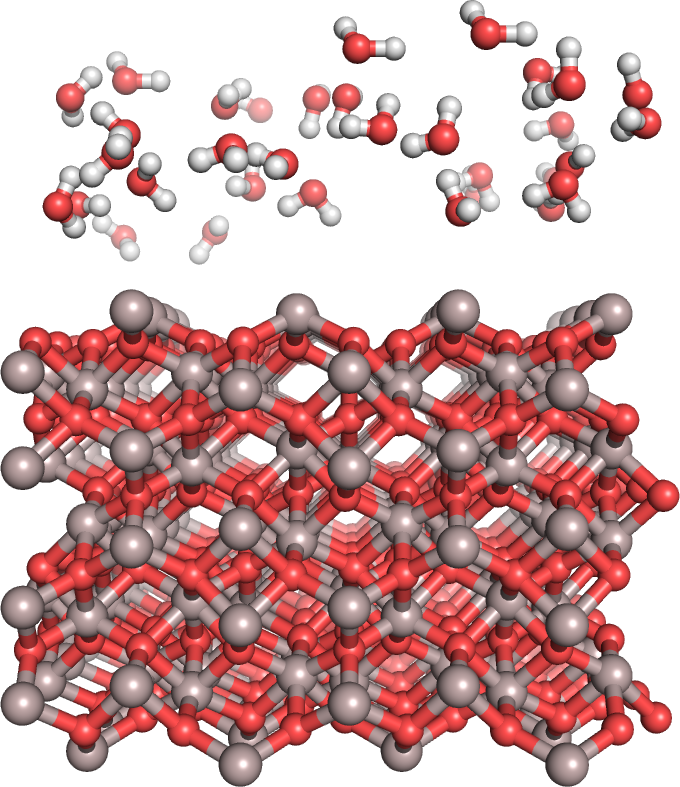
\includegraphics[width=\textwidth]{AlO_first_transparent}
    \subcaption{Seitenansicht, \\
      vor der Reaktion}
    \label{fig:wateraluminasurface-a}
  \end{subfigure}
  \hfill
  \begin{subfigure}[t]{\subfigwidth}
    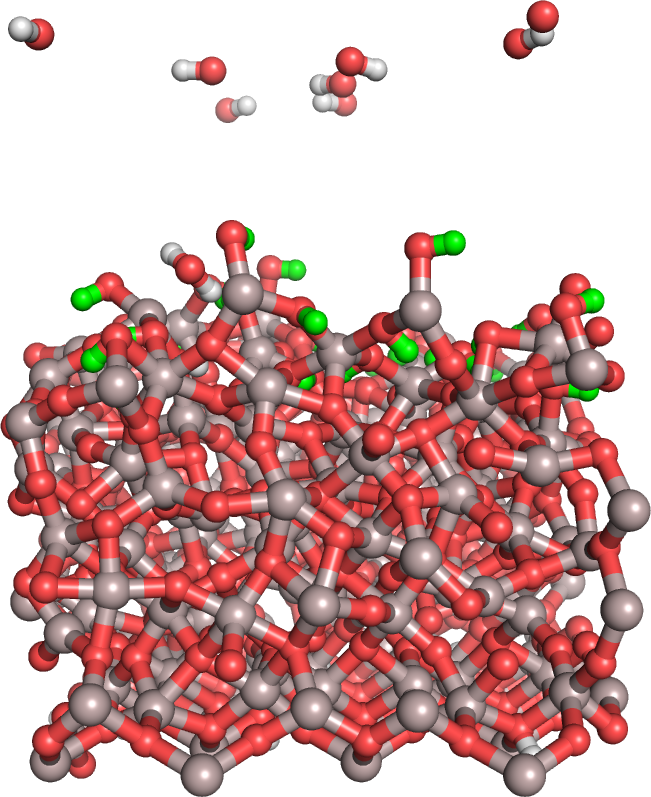
\includegraphics[width=\textwidth]{AlO_hydroxylation_side}
    \subcaption{Seitenansicht, \\
      nach der Reaktion}
    \label{fig:wateraluminasurface-b}
  \end{subfigure}
  \hfill
  \begin{subfigure}[t]{\subfigwidth}
    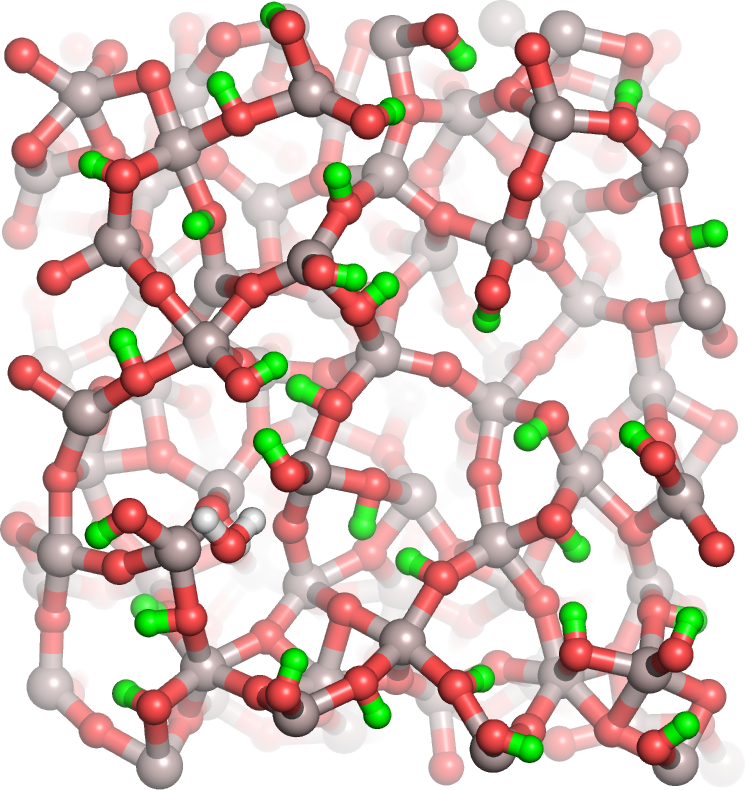
\includegraphics[width=\textwidth]{AlO_hydroxylation_top_transparent_thinner}
    \subcaption{Draufsicht,\\
      nach der Reaktion
    }
    \label{fig:wateraluminasurface-c}
  \end{subfigure}
  \caption{
    Simulation einer Hydroxylierung von $\alpha$-\ce{Al2O3} mit Wasser.
    Die Oberfläche wird mit Hydroxylgruppen (grün hervorgehoben) abgesättigt.
  }
  \label{fig:wateraluminasurface}
\end{figure}

Mit den \pot{narayanan}-Parametern konnten keine Adsorptionen beobachtet werden, da sie in den Simulationen durch eine repulsive Kraft zwischen den Wassermolekülen und der Oberfläche verhindert werden.
Das deutet darauf hin, dass Hydroxylgruppen auf einer Aluminiumoxid-Oberfläche von dem Parametersatz energetisch nicht bevorzugt werden oder die Adsorptionen mit übermäßig hohen Reaktionsbarrieren verbunden sind.

Das Ergebnis der Simulationen für die \pot{liu}-Parameter (Abbildungen~\ref{fig:wateraluminasurface-b} und~\ref{fig:wateraluminasurface-c}) zeigt jedoch die gleichmäßige Bedeckung der Oberfläche mit Hydroxylgruppen neben gelegentlich adsorbierten Wassermolekülen, die keine Oberflächenreaktion eingegangen sind.
Letztere sollten sich aber auf längere Sicht durch die Einflüsse der Überkoordinationsterme des ReaxFF-Potentiales von der Oberfläche lösen oder eine Reaktion mit benachbarten Sauerstoff-Atomen eingehen.
Die Hydroxyl-Bedeckung der Oberfläche stimmt dabei mit \SI{9.5}{\per\square\nano\meter} mit den Referenzwerten von \SI{9.2}{\per\square\nano\meter} überein, wodurch die Sättigung der Oberfläche mit Hydroxylgruppen bestätigt wird.
Einige der Atome in Abbildung~\ref{fig:wateraluminasurface} sind scheinbar stark überkoordiniert, doch werden die Bindungen für die Visualisierung aus den Nachbarschaftsbeziehungen der Atome generiert und sind nicht repräsentativ für die Beschreibung der Bindungen durch ReaxFF.
Die überschüssigen Wassermoleküle sind in der Gasphase verblieben, wie in Abbildung~\ref{fig:wateraluminasurface-b} am oberen Rand des periodischen Simulationsraumes erkennbar ist, bei denen sie durch periodische Randbedingungen zerteilt erscheinen.
Es konnte damit gezeigt werden, dass die Begrenzung der Reaktion von Wasser durch die sterische Hinderung der Wassermoleküle in der Simulation wiedergegeben wird.


\subsection{Fazit}

Mit dem \pot{liu}-Parametersatz konnte neben Eigenschaften der Bulkmaterialien auch die selbstsättigende Hydroxylierung einer $\alpha$-kristallinen \ce{Al2O3}-Ober\-fläche durch die chemische Adsorption von Wassermolekülen simuliert werden.
Eine vollständige Beschreibung des TMA-\ce{H2O}-ALD-Prozesses ist jedoch mit keiner der untersuchten Parametrisierungen möglich.
